\chapter{Detección}
\label{Ch:4}
\graphicspath{{figs/}}
%%%%%%%%%%%%%%%%%%%%%%%%%%%%%%%%%%%%%%%%%%%%%%%%%%%%%%%%%%%%%%%%%%%%%%%%

\section{Prueba de Hipótesis}
\label{S:prueba-hipotesis}

El problema de detección se resolverá por medio de un test de hipótesis sobre una ventana de evaluación $\mathbf{y}$, de $N$ muestras en donde $N$ es la longitud de la secuencia de entrenamiento de símbolos cortos. La ventana representa las últimas $N$ muestras recibidas por el receptor.
\begin{equation}\label{eq:def_y}
    \mathbf{y} = \begin{bmatrix}
        y[0] & y[1] & \cdots & y[N-1]
    \end{bmatrix}
\end{equation}

Los pasos para realizar el test son los siguientes
\begin{enumerate}
    \item Definición de dos o más hipótesis mutuamente excluyentes acerca del orígen de las muestras observadas.
    \item Definición de un estadístico en función de las muestras bajo estudio, que recibe el nombre $\phi\left[\mathbf{y}\right]$.
    \item Definición de una regla de decisión sobre el estadístico elegido para discriminar entre las hipótesis disponibles según determinado criterio. 
    \item Estimación de los parámetros necesarios para aplicar la regla de decisión
\end{enumerate}

\subsection{Definición de Hipótesis}
\label{Ss:def-hipotesis}

Se definen dos hipótesis sobre el origen de las muestras, estas reciben el nombre de hipótesis nula ($H_0$) e hipótesis alternativa ($H_1$), y son las siguientes:
\begin{itemize}
    \item $H_0$, el intervalo de evaluación contiene únicamente ruido.
    \item $H_1$, el intervalo de evaluación contiene una secuencia de entrenamiento de símbolos cortos afectada por ruido aditivo y modificada por el canal inalámbrico.
\end{itemize}

Se hacen varias suposiciones en las definiciónes de las hipótesis
\begin{itemize}
    \item Las muestras de ruido siguen la distribución normal compleja, son independientes, e idénticamente distribuidas. 
    \item La respuesta al impulso del canal puede ser aproximada por un único \textit{tap}, por lo que cada muestra de la secuencia transmitida se puede ver modificada por un factor de amplitud y fase, pero no influye en las muestras anteriores ni siguientes.
    \item El canal presenta desvanecimiento lento, por lo que el factor que modifica la amplitud y fase de una señal recibida se mantiene aproximadamente constante.
\end{itemize}

Tomando en cuenta las suposiciones, se procede a formalizar la expresión matemática de las hipótesis
\begin{equation}\label{eq:def-hipótesis}
    \begin{aligned}
        H_0&: \quad \mathbf{y} = \mathbf{w}\\
        H_1&: \quad \mathbf{y} = A\mathbf{s} + \mathbf{w}
    \end{aligned}
    \qquad\qquad
    \mathbf{w} \sim \mathcal{CN}\left[\mathbf{0},\, \sigma^2 I_N\right]
\end{equation}

En donde $\mathbf{s}$ es la secuencia de entrenamiento de símbolos cortos, de $N$ muestras de longitud, y $A$ es un factor complejo incógnito pero constante que modifica la amplitud y fase de la secuencia.	

\subsubsection{Definición de SNR}

En el caso de que la hipótesis alternativa sea verdadera, resulta conveniente definir una medida de la relación señal a ruido. La definición utilizada es el cociente entre la potencia media de una muestra de señal y la potencia media de una muestra de ruido.
\begin{equation}\label{eq:snr-definicion}
\text{SNR} = \frac{\text{Potencia media señal}}{\text{Potencia media ruido}}
\end{equation}

Las suposiciones hechas implican que la potencia media de la señal es un valor determinista
\begin{equation}\label{eq:potencia-señal}
\overline{P}_s = \frac{1}{N}\sum_{k=0}^{N-1}\lvert A s[k] \rvert^2 = \frac{1}{N} \lvert A \rvert^2 \lVert \mathbf{s} \rVert^2
\end{equation}

La potencia media del ruido surge de las propiedades estadísticas de su distribución, y se calcula a partir de la propiedad del módulo de una variable aleatoria normal compleja, el cual sigue una distribución Rayleigh
\begin{equation}
w[k] \sim \mathcal{CN}\left[0, \sigma^2\right]  \implies|w[k]| \sim \mathcal{R}ay\left[\sigma\right],
\end{equation}

y el hecho de que media de la distribución Rayleigh es conocida, así como lo es su varianza
\begin{equation}
E\left[\lvert w[k]\rvert\right] = \sigma \sqrt{\frac{\pi}{2}}\qquad\qquad V[\left\lvert w[k] \rvert\right] = \frac{4-\pi}{2} \sigma^2
\end{equation}

Lo cual permite calcular la potencia media de una muestra de ruido de la siguiente forma
\begin{equation}\label{eq:potencia-ruido}
E\left[\lvert w[k]\rvert^2\right] = V\left[\lvert w[k]\rvert\right] + E\left[\lvert w[k]\rvert\right]^2 =  2\sigma^2
\end{equation}

Remplazando los valores obtenidos de las Ecuaciones \ref{eq:potencia-señal} y \ref{eq:potencia-ruido} en la Ecuación \ref{eq:snr-definicion} se obtiene la expresión de la SNR cuando la hipótesis alternativa es verdadera
\begin{equation}
\text{SNR} = \frac{\frac{1}{N} A^2 \lVert \mathbf{s} \rVert ^2}{2 \sigma^2}
\end{equation}

\subsection{Elección de Estadístico}
\label{Ss:hipotesis-estadistico}


El estadístico utilizado será el mismo que se calcula en el algoritmo de sincronismo con banco de correladores, la correlación con la secuencia de entrenamiento de símbolos cortos. Por practicidad se expresará de la siguiente forma
\begin{equation}
    \phi[\mathbf{y}] = \left\lvert\sum_{k=0}^N s^\ast[k]y[k]\right\rvert = \lvert \mathbf{s}^\ast\mathbf{y}\rvert
\end{equation}

Al momento de estudiar las propiedades estadísticas de $\phi$ resulta conveniente trabajar con un resultado intermedio, el cual es el valor complejo de la correlación previo a la operación módulo.
\begin{equation}
    \psi[\mathbf{y}] = \sum_{k=0}^N s^\ast[k]y[k] = \mathbf{s}^\ast\mathbf{y}
\end{equation}

\subsection{Distribución del estadístico ante hipótesis nula}

Se estudia la distribución del estadístico $\psi$ en el caso que $\mathbf{y}$ es únicamente ruido

\begin{equation}\label{eq:psi-ante-h0}
    \mathbf{y} | H_0 = \mathbf{w} \implies \psi[\mathbf{y}] | H_0= \sum_{k = 0}^{N-1} s^\ast[k]w[k]
\end{equation}

En estas condiciones, se observa que $\psi$ resulta una sumatoria de muestras de ruido, cada muestra escalada por su correspondiente término de la secuencia de entrenamiento de símbolos cortos. Esto resulta en una sumatoria de variables normales complejas de diferente varianza
\begin{equation}
    s^\ast[k]w[k] \sim \mathcal{CN}[0,\, \lvert s[k]\rvert^2\sigma^2]
\end{equation}

Finalmente, aplicando la propiedad de la suma de variables aleatorias gausianas

La cual se puede reducir a la siguente expresión
\begin{equation}
    \begin{aligned}
        \psi | H_0 &\sim \mathcal{CN}\left[0,\, \sum_{k=0}^{N-1} \lvert s[k]\rvert^2  \sigma^2 \right]\\[0.5em]
        \psi | H_0 &\sim \mathcal{CN}\left[0,\,\lVert \mathbf{s}\rVert^2  \sigma^2 \right] 
    \end{aligned}
\end{equation}

Tal como se ha visto anteriormente, el módulo de de una distribución normal compleja sigue una distribución Rayleigh, por lo que conocemos la distribución de $\phi$ condicionada por $H_0$. Por conveniencia expresamos con la función de probabilidad acumulada
\begin{equation}\label{eq:phi-ante-h0}
    F_\phi(\phi|H_0) = 1- \exp\left[-\frac{\phi^2}{2\lVert\mathbf{s}\rVert^2 \sigma^2}\right]    
\end{equation}


\subsection{Distribución del estadístico ante hipótesis alternativa}

Nuevamente se parte de la distribución de $\psi$, en este caso cuando la hipótesis alternativa es verdadera.
\begin{equation}\label{eq:psi-ante-h1}
    \begin{aligned} 
        \mathbf{y} | H_! = A\mathbf{s} + \mathbf{w} \implies \psi[\mathbf{y}] | H_1  
        &= \mathbf{s}^\ast\left(A\mathbf{s}+\mathbf{w}\right)\\ 
        &= A\lVert\mathbf{s}\rVert^2+\mathbf{s}^\ast\mathbf{w}
    \end{aligned}
\end{equation}

Es evidente la similitud de este caso con el estudiado anteriormente. La ecuación \ref{eq:psi-ante-h1} describe la suma de un término determinista y un término aleatorio, el efecto del término determinista es únicamente el de desplazar la media de la distribución.
\begin{equation}
    \psi | H_1 \sim \mathcal{CN}\left[A\lVert\mathbf{s}\rVert^2,\,\lVert \mathbf{s}\rVert^2  \sigma^2 \right] 
\end{equation}

Nuevamente $\psi$ sigue una distribución normal compleja, pero en este caso ya no es de media nula. Para proceder se normaliza la variable aleatoria, definiendo una nueva variable aleatoria $\psi'$ que tendrá varianza unitaria.
\begin{equation}
    \psi' = \frac{\psi}{\lVert \mathbf{s} \rVert \sigma} \quad \implies \quad     \psi' | H_1 \sim \mathcal{CN}\left[\frac{A\lVert\mathbf{s}\rVert}{\sigma},\, 1 \right] 
\end{equation}

Con el mismo factor de normalización definiremos $\phi'$.
\begin{equation}
\phi' = \frac{\phi}{\lVert \mathbf{s} \rVert \sigma} \quad \longrightarrow \quad     \phi' = \lvert\psi'\rvert
\end{equation}

El propósito de la normalización es que esta permite utilizar la definición de la distribución $\chi$ no central\cite{distributions}, la cual es definida de la siguiente forma. Si existen $n$ variables aleatorias normales $x_i$ independientes de varianza unitaria y respectivas medias $\mu_i$, y se define $z$ como la raiz de la sumatoria de sus cuadrados
\begin{equation}
    z = \sqrt{\sum_{i=1}^{n}x_i^2}
\end{equation}

Esta variable seguirá la distribución $\chi$ no central de $n$ grados de libertad y parámetro de no-centralidad $\lambda$, el cual es calculado de la siguiente forma
\begin{equation}
    \lambda = \sqrt{\sum_{i=1}^{n}\mu_i^2}
\end{equation}

Esta definición se puede aplicar a nuestro problema para encontrar la distribución de $\phi'$, en tal caso tendremos $n = 2$, $x_1$ y $x_2$ son la parte real e imaginaria de $\psi'$ respectivamente, y $\mu_1$ y $\mu_2$ son la parte real e imaginaria de su media compleja. Se obtiene el parámetro $\lambda$
\begin{equation}
    \displaystyle\mu_1 = \frac{\rVert\mathbf{s}\rVert}{\sigma}\mathcal{R}e\left[A\right] \quad \displaystyle\mu_2 = \frac{\rVert\mathbf{s}\rVert}{\sigma}\mathcal{I}m\left[A\right] \quad \implies \quad \lambda = \frac{\lVert\mathbf{s}\rVert}{\sigma}\lvert A \rvert
\end{equation}

Resulta la distribución
\begin{equation}
    \phi' | H_1 \sim \chi_{NC}\left[n = 2, \, \lambda = \frac{|A|\lVert\mathbf{s}\rVert}{\sigma}\right] 
\end{equation}

Tal como es el caso anterior, se continúa trabajando con la función de probabilidad acumulada
\begin{equation}
    F_{\phi'}(\phi'|H_1) = 1-\int_{\phi'}^\infty x\exp\left[-\frac{x^2 + \frac{|A|^2\lVert\mathbf{s}\rVert^2}{\sigma^2}}{2}\right]I_0\left[\frac{|A|\lVert\mathbf{s}\rVert}{\sigma} x\right] dx
\end{equation}

Finalmente, se aplica el cambio de variables para revertir la normalización, obteniendo la distribución acumulada de $\phi$ ante la hipótesis alternativa
\begin{equation}\label{eq:phi-ante-h1}
    F_\phi(\phi|H_1) = 1-\int_{\frac{\phi}{\lVert\mathbf{s}\rVert\sigma}}^\infty x\exp\left[-\frac{x^2 + \frac{|A|^2\lVert\mathbf{s}\rVert^2}{\sigma^2}}{2}\right]I_0\left[\frac{|A|\lVert\mathbf{s}\rVert}{\sigma} x\right] dx
\end{equation}

\subsection{Regla de Decisión}
\label{Ss:hipotesis-umbral}\label{eq:def-pfa}

La regla de decisión típica en los casos que se cuentan con dos hipótesis es la comparación del estadístico con un umbral $T$, tal que si el estadístico excede el umbral se decide por la hipótesis alternativa, mientras que si no lo hace se opta por la hipótesis nula.
\begin{equation}
    \phi[\mathbf{y}]\mathop{\lessgtr}_{H_1}^{H_0}T
\end{equation}

En función del estadístico y el umbral se definen la probabilidad de Falsa Alarma $P_{FA}$, que es la probabilidad de decidir por la hipótesis alternativa cuando la hipótesis nula es verdadera
\begin{equation}
    P_{FA} = \int_T^\infty f_\phi(\phi|H_0)d\phi = 1 - F_\phi(T|H_0)    
\end{equation}

Asimismo se define la probabilidad de Detección $P_D$, la cual es probabilidad de decidir por la hipótesis alternativa cuando esta efectivamente es verdadera
\begin{equation}
    P_{D} = \int_T^\infty f_\phi(\phi|H_1)d\phi = 1 - F_\phi(T|H_1)
\end{equation}

El criterio elegido para la elección del umbral es tal que la probabilidad de falsa alarma se mantenga constante a un valor elegido. Tomando la expresión de $F_\phi(\phi|H_0)$ calculado en la ecuación \ref{eq:phi-ante-h0}, y remplazándolo en la ecuación \ref{eq:def-pfa} se obtiene
\begin{equation}
    P_{FA} = \exp\left[-\frac{T^2}{2\lVert\mathbf{s}\rVert^2 \sigma^2}\right]    
\end{equation}

Despejando se obtiene la función para determinar el umbral que obtendrá la probabilidad de falsa alarma deseada
\begin{equation}\label{eq:umbral}
    T(P_{FA}) = \sqrt{-2\lVert \mathbf{s}\rVert^2 \sigma^2 \ln\left[P_{FA}\right]}    
\end{equation}

\subsection{Desempeño}
\label{Ss:hipotesis-desempeño}
Se estudian dos medidas de desempeño, las cuales surgen de evaluar la probabilidad de detección. Para medirlas se busca $P_D$ a partir de reemplazar $F_\phi(\phi|H_1)$ calculado en la ecuación \ref{eq:phi-ante-h1} y el valor del umbral calculado en la ecuación \ref{eq:umbral}
\begin{equation}\label{eq:probabilidad-deteccion}
    P_D = \int_{\sqrt{-2 \ln\left[P_{FA}\right]}}^\infty x\exp\left[-\frac{x^2 + \frac{|A|^2\lVert\mathbf{s}\rVert^2}{\sigma^2}}{2}\right]I_0\left[\frac{|A|\lVert\mathbf{s}\rVert}{\sigma} x\right] dx
\end{equation}

Al observar la expresión de la probabilidad de detección resultante, se nota que tanto $A$ como $\sigma$ solo influyen en esta a través de la relación entre estos, lo cual es un resultado razonable. Esto incentiva a expresar la probabilidad de detección en función de la SNR, calculada anteriormente en la ecuación \ref{eq:snr-definicion}.
\begin{equation}\label{eq:probabilidad-deteccion-snr}
    P_D = \int_{\sqrt{-2 \ln\left[P_{FA}\right]}}^\infty x\exp\left[-\frac{x^2 + 2N\,\text{SNR}}{2}\right]I_0\left[\sqrt{2N\,\text{SNR}}\,x\right] dx
\end{equation}

Al expresarlo así se nota que la probabilidad de detección depende de la probabilidad de falsa alarma elegida, y de la relación señal a ruido presente en la señal. De esa dependencia se pueden evaluar dos medidas de desempeño, la probabilidad de detección en función de la probabilidad de error a SNR constante, y la probabilidad de detección en función de la SNR a probabilidad de falsa alarma constante. Estas métricas de desempeño se validan con simulaciones numéricas, las cuales se realizan de la siguiente forma. 

\begin{itemize}
    \item Se fija un par de valores de $P_{FA}$ y SNR. Se determinan arbitrariamente valores de $A$ y $\sigma^2$ que resulten en el SNR elegido al aplicar la Ecuación \ref{eq:snr-definicion}, y se calcula el valor de $T$.
    \item Se calcula el valor esperado teóricamente de $P_D$ con la Ecuación \ref{eq:probabilidad-deteccion-snr}, la cual se resuelve con integración numérica.
    \item Para tener un número de realizaciones razonables pero estadísticamente representativo del experimento, se elige hacer $100/P_D$ realizaciones.
    \item En cada realización se genera un vector de $N$ muestras $\mathbf{y} = A\mathbf{s}+\mathbf{w}$ con los valores de $A$ y $\sigma^2$ elegidos anteriormente. 
    \item Se calcula $\phi$ sobre ese vector y se compara con $T$. Si resulta $\phi > T$ se registra una detección.
    \item Una vez terminadas las realizaciones, la probabilidad de detección empírica es el número de detecciones dividido por el número total de realizaciones.
\end{itemize}

\begin{figure}[t]
    \centering{}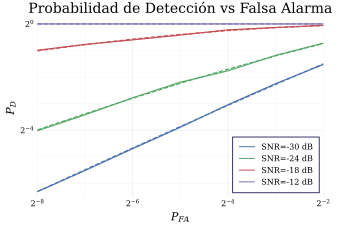
\includegraphics[width=\imsize]{pd_vs_pfa.svg}
    \caption{Asignación de subportadoras para la construcción de la secuencia de entrenamiento de símbolos largos.\label{fig:pdd-vs-pfa}}
\end{figure}
\begin{figure}[t]
    \centering{}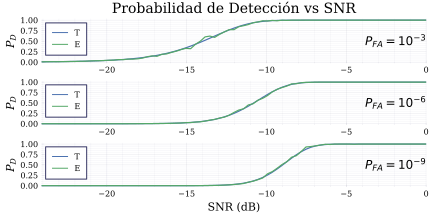
\includegraphics[width=\imsize]{pd_vs_snr.svg}
    \caption{Secuencia de entrenamiento de símbolos largos en el dominio temporal, usando $T_{LONG} = 8$ \textmu s y una IFFT de 64 puntos..\label{fig:pd-vs-snr}}  
\end{figure}


%Y derivando
%
%\begin{equation}
%    f_\phi(\phi|H_1) = \frac{\phi}{\lVert\mathbf{s}\rVert^2\sigma^2} \exp\left[-\frac{\phi^2 + A^2\lVert\mathbf{s}\rVert^4}{2\lVert\mathbf{s}\rVert^2\sigma^2}\right]I_0\left[\frac{A}{\sigma^2}\phi\right] dx
%\end{equation}

\section{Estimación del Ruido}
\label{S:estimacion-ruido}

Para estimar la varianza del ruido, se selecciona el estimador insesgado de mínima varianza (MVUE por sus siglas en inglés). El método para encontrarlo es usando el teorema de Rao-Blackwell-Lehmann-Scheffe. \cite{kay}

El procedimiento requiere de un estadístico suficiente para un parámetro de la distribución de ciertos datos obtenidos. 
Los datos se suponen provenientes de ruido normal complejo de media nula independientes e idénticamente distribuidos, se le asigna el nombre $\mathbf{w}$ y su distribución será la siguiente. 
\begin{equation}\label{eq:noise-estimation-distribution}
    f(\mathbf{w}) = \frac{1}{\left(\pi\sigma^2\right)^N} \exp\left[- \frac{\mathbf{w}^\ast \mathbf{w}}{\sigma^2}\right]
\end{equation}

El teorema establece que si uno encuentra una función de un estadístico suficiente que retorne un estimador insesgado del parámetro, este será el MVUE. 

Para obtener el estadístico suficiente, se utiliza el teorema de factorización de Neyman--Fischer establece que si la distribución de probabilidad de $\mathbf{w}$ puede ser expresada como el producto
\begin{equation}
    f(\mathbf{w}, \sigma^2) = g(T(\mathbf{w}), \sigma^2)h(\mathbf{w})
\end{equation}

Entonces $T(\mathbf{w})$ es un estadístico suficiente para $\sigma^2$. Efectivamente la distribución tal como es descrita en la ecuación \ref{eq:noise-estimation-distribution} tiene esta forma si se eligen las siguientes funciones
\begin{equation}
    h(\mathbf{w}) = 1 \qquad\qquad T(\mathbf{w}) = \mathbf{w}^\ast \mathbf{w}
\end{equation}

Para obtener una función de $T(\mathbf{w})$ que retorne un estimador insesgado, resulta util calcular el valor esperado de $T(\mathbf{w})$, lo cual en este caso es fácil ya que las muestras son independientes e idénticamente distribuidas. 
\begin{equation}
    E\left[\mathbf{w}^\ast\mathbf{w}\right] =  E\left[\sum_{i=0}^{N-1}\lvert w[i]\rvert^2\right]  =   \sum_{i=0}^{N-1}E\left[\lvert w[i]\rvert^2\right] 
\end{equation}

El valor esperado del módulo al cuadrado de una muestra de ruido fue calculado anteriormente, en la sección \ref{Ss:def-hipotesis}. De esta forma se obtiene 
\begin{equation}
    E\left[\mathbf{w}^\ast\mathbf{w}\right] =  \sum_{i=0}^{N-1}2\sigma^2 = 2N\sigma^2 
\end{equation}

Conociendo ese valor, puede calcular facilmente una función que retorne un estadístico insesgado aplicando un factor de correción multiplicativo, esta función será el MVUE.
\begin{equation}
    \widehat{\sigma^2}_{MVU} = g\left(\mathbf{w}^\ast\mathbf{w}\right) =  \frac{\mathbf{w}^\ast\mathbf{w}}{2N}
\end{equation}



\section{Resultados}
\label{S:deteccion-resultados}



%%% Local Variables: 
%%% mode: latex
%%% TeX-master: "template"
%%% End: 
